\documentclass[11pt, english]{article}
\usepackage{graphicx}
\usepackage[colorlinks=true, linkcolor=blue]{hyperref}
\usepackage[spanish]{babel}
\selectlanguage{english}
\usepackage[utf8]{inputenc}
\usepackage[svgnames]{xcolor}
\usepackage{booktabs}

\usepackage{listings}
\usepackage{afterpage}

\pagestyle{plain}

\definecolor{dkgreen}{rgb}{0,0.6,0}
\definecolor{gray}{rgb}{0.5,0.5,0.5}
\definecolor{mauve}{rgb}{0.58,0,0.82}
%\lstset{language=R,
%    basicstyle=\small\ttfamily,
%   stringstyle=\color{DarkGreen},
%    otherkeywords={0,1,2,3,4,5,6,7,8,9},
%    morekeywords={TRUE,FALSE},
%    deletekeywords={data,frame,length,as,character},
%    keywordstyle=\color{blue},
%    commentstyle=\color{DarkGreen},
%}

\lstset{frame=tb,
language=R,
aboveskip=3mm,
belowskip=3mm,
showstringspaces=false,
columns=flexible,
numbers=none,
keywordstyle=\color{blue},
numberstyle=\tiny\color{gray},
commentstyle=\color{dkgreen},
stringstyle=\color{mauve},
breaklines=true,
breakatwhitespace=true,
tabsize=3,
escapeinside={(@}{@)}
}

\usepackage{here}


\textheight=21cm
\textwidth=17cm
%\topmargin=-1cm
\oddsidemargin=0cm
\parindent=0mm
\pagestyle{plain}

%%%%%%%%%%%%%%%%%%%%%%%%%%
% La siguiente instrucción pone el curso automáticamente%
%%%%%%%%%%%%%%%%%%%%%%%%%%

\usepackage{color}
\usepackage{ragged2e}

\global\let\date\relax
\newcounter{unomenos}
\setcounter{unomenos}{\number\year}
\addtocounter{unomenos}{-1}
\stepcounter{unomenos}
\gdef\@date{ Curso  2018 / \arabic{unomenos}}

\begin{document}

\begin{titlepage}

\begin{center}
\vspace*{-1in}
\begin{figure}[htb]
\begin{center}
\includegraphics[width=10cm]{../res/pics/logo.jpg}
\end{center}
\end{figure}

\vspace*{0.4in}
\begin{large}
\textsc{Procesadores de Lenguaje}:\\
\end{large}
\vspace*{0.2in}
\begin{Large}
\textbf{\textsc{Nombre de nuestro lenguaje}} \\
\end{Large}
\vspace*{0.3in}
\begin{large}
\@date\\
\end{large}
\vspace*{0.3in}
\rule{80mm}{0.1mm}\\
\vspace*{0.1in}
\begin{large}
Realizado por: \\

Medina Medina, David Alberto  \\
Brito Ramos, Christian  \\
Hernández Delgado, Christopher \\
López González, Néstor \\
\vspace*{0.3in}
\end{large}

\includegraphics[width=3cm]{../res/pics/LogoEscuela.jpg}
\end{center}
\end{titlepage}

\newcommand{\CC}{C\nolinebreak\hspace{-.05em}\raisebox{.4ex}{\tiny\bf +}\nolinebreak\hspace{-.10em}\raisebox{.4ex}{\tiny\bf +}}
\def\CC{{C\nolinebreak[4]\hspace{-.05em}\raisebox{.4ex}{\tiny\bf ++}}}

\tableofcontents
\newpage

\section{Definición del lenguaje (Autor: Quien termine antes)}
Introducir breve introducción del lenguaje que planteamos.
\newpage

\subsection{Tipos de datos (David)}
Cualquier leguaje de programación necesita definir un conjunto de \emph{tipos de datos}, esto es, la batería de valores y operaciones que puede adquirir una variable. Cada tipo de dato está definido en el lenguaje por un \emph{literal} único que lo representa, lo que permite que cada tipo de dato tenga un representación física específica.

Los tipos de datos definidos en el lenguaje son los que figuran en el \emph{cuadro \ref{tab:table1}}. Las características críticas de implementación que define a cada tipo son:

\begin{description}
	\item[Entero] Representa a todas y cada una de las variables enteras que sean declaradas en el lenguaje. Este tipo de dato presenta un tamaño de 4 bytes (32 bits) y permite representar números enteros con signo. El \emph{complemento a 2} es el sistema elegido para definir el signo del número entro. Este dato se representa por el literal \texttt{int}. El rango de valores que puede tomar es 
	
	\begin{equation}\label{eq:equation1}
		\left [-2^{N-1},\: 2^{N-1}-1 \right ] = \left [-2^{32-1},\: 2^{32-1}-1 \right] = \left [-2147483648,\: 2147483647 \right]
	\end{equation}
	
	donde, $N$ es el número de bits disponibles para representar el número el número entero (32 bits).
	\item[Coma flotante de simple precisión] Este tipo de dato representa número reales en coma flotante de simple precisión con un tamaño de 4 bytes (32 bits) siguiendo el estándar \emph{IEEE 754}. En la figura \ref{fig:figure1} puede observarse como esta representación binaria los bits se organizan en tres sectores principales:
	\begin{itemize}
		\item \textbf{Signo} (1 bit). Se trata de un sólo bit que define el signo del número: positivo (0) o negativo (1).
		\item  \textbf{Exponente (8bits)}. Se trata de un número entero con signo de complemento a 2 ($\left [ -128,\: 127\right ]$)
		\item \textbf{Mantisa (23 bits)}. Conforma la fracción a la derecha de la coma binaria y un bit de encabezado implícito.
	\end{itemize}
	Este tipo de dato se representa con el literal \texttt{real}. Su rango de valores es de $\left [ 1.18 \cdot 10^{–38},\; 3.4 \cdot 10^{38} \right ]$.
	\begin{figure}[H]\label{fig:figure1}
		\centering
		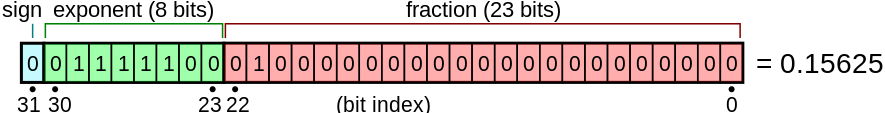
\includegraphics[width=0.75\textwidth]{../res/pics/data-types/float_diag.png}
		\caption{Representación binaria de número en coma flotante de simple precisión (\emph{IEEE 754})}
	\end{figure}

	\item[Caracter] Este tipo de dato es usado para representar caracteres de codificación \emph{UTF-8}, es por este motivo que el tamaño de que ocupan las variables de tipo caracter son de 4 bytes siendo \texttt{char} el literal que lo representa.
	\item[Booleano] Se trata de un tipo de dato utilizado para representar representar valores booleanos. Su tamaño es de 1 bit, por lo que tan solo puede tomar dos valores: \texttt{1} (verdadero) ó \texttt{0} (falso). El literal que lo representa es \texttt{bool}.
\end{description} 

\begin{table}[h!]
	\begin{center}
		\caption{Tipos de datos}
		\label{tab:table1}
		\begin{tabular}{l|l|l|l}
			\toprule
			\textbf{Tipo} & \textbf{Literal} & \textbf{Tamaño} & \textbf{Rango}\\
			\midrule
			Entero & int &4 Bytes & $\left [-2147483648,\: 2147483647 \right]$\\
			Coma flotante de simple precisión & real & 4 Byte & $\left [ 1.18 \cdot 10^{–38},\; 3.4 \cdot 10^{38} \right ]$\\
			Caracter & char & 1 Byte & \emph{UTF-8}\\
			Lógico & bool & 1 Bit & $\left [0,\; 1 \right ]$\\
			\bottomrule
		\end{tabular}
	\end{center}
\end{table}

En el siguiente ejemplo se muestra cómo se declaran las variables con los literales de los tipos descritos anteriormente:

\lstinputlisting[language=C++]{../res/lst/data-types/data-type.x}

\subsection{Colecciones de datos: \texttt{Arrays}}
Las variables pueden ser agrupadas en colecciones de datos de una dimensión denominados \emph{arrays}. En este lenguaje, cualquier tipo de dato puede formar parte de un \emph{array}.

% Añadir listado de ejemplo
\newpage

\subsection{Palabras reservadas (Christian)}
Aquí va el texto. Poner siempre un código de ejemplo.
\newpage

\subsection{Comentarios (Christian)}
Aquí va el texto. Poner siempre un código de ejemplo.
\newpage

\subsection{Tipos de operadores}
Aquí va el texto. Poner siempre un código de ejemplo.

\subsubsection{Operadores aritméticos (David)}
Aquí va el texto. Poner siempre un código de ejemplo.
\newpage

\subsubsection{Operadores lógicos (Christopher)}
Definimos los símbolos que identificarán a los operadores lógicos de forma análoga a los utilizados por gran parte de otros lenguajes de programación, separando cada operador 2 expresiones a comparar por los operadores lógicos a utilizar, con la excepción del propio \emph{NOT}, que podrá utilizarse directamente para determinar si el valor devuelto por una expresión de tipo \texttt{booleano} es directamente verdadero o no. Como dato adicional, también consideramos la posibilidad de hacer uso de comparadores mediante dichos operadores lógicos n-arios, comparando pares de expresiones entre sí de forma sucesiva siguiendo el orden de lectura de izquierda a derecha (que a efectos prácticos es lo mismo que hacer sucesivos \emph{AND} pero de forma más breve) y la posibilidad de prioridades para ciertos operadores (como el \emph{AND}). \vspace{0px}

En relación a las expresiones de comparación, consideramos hacer que de momento solo se puedan utilizar entre tipos de datos del mismo tipo o similar (por ejemplo, entre enteros y reales podría hacerse). Dejamos la tabla de operadores como sigue: \vspace{0px}
\begin{table}[h!]
	\begin{center}
		\caption{Tipos de operadores lógicos}
		\label{tab:table2}
		\begin{tabular}{c|c|c|c}
		\toprule
		\multicolumn{1}{c}{\textbf{Operador}} & \multicolumn{1}{c}{\textbf{Símbolo}} & \multicolumn{1}{c}{\textbf{Formato}}      & \multicolumn{1}				{c}{\textbf{Tipos de datos comparables}}            
		\\ \midrule
		AND                            & \&\&                         & \{EXPR\} \&\& \{EXPR\}            & LOGICO - LOGICO                                                                                                                                  		\\ \midrule
		OR                             & \textbar\textbar                           & \{EXPR\} \textbar\textbar$ \; $\{EXPR\}              & LOGICO - LOGICO                                                                                                                                  		\\ \midrule
		NOT                            & !                            & !\{EXPR\}                         & LOGICO                                                                                                                                           		\\ \midrule
		IGUAL                          & ==                           & \{EXPR\} == \{EXPR\}              & \begin{tabular}[c]{@{}c@{}}LOGICO - LOGICO \\ ENTERO - 		ENTERO  \\  ENTERO - REAL  \\ REAL - REAL  \\  CHAR - CHAR  \\ ARRAY{[}CHAR{]} - ARRAY{[}CHAR{]}\end{tabular} \\ \midrule
		NOIGUAL                        & !=                           & \{EXPR\} != \{EXPR\}              & \begin{tabular}[c]{@{}c@{}}LOGICO - LOGICO \\ ENTERO - 		ENTERO  \\  ENTERO - REAL  \\ REAL - REAL  \\  CHAR - CHAR  \\  ARRAY{[}CHAR{]} - ARRAY{[}CHAR{]}\end{tabular} \\ \midrule
		MAYOR                          & \textgreater{}               & \{EXPR\} \textgreater $ \; $\{EXPR\}    & \begin{tabular}[c]{@{}c@{}}ENTERO - ENTERO  \\  		ENTERO - REAL \\ REAL - REAL\end{tabular}                                                                \\ \midrule
		MAYORIGUAL                     & \textgreater{}=              & \{EXPR\} \textgreater{}= \{EXPR\} & \begin{tabular}[c]{@{}c@{}}ENTERO - ENTERO  \\  		ENTERO - REAL \\ REAL - REAL\end{tabular}                                                                      
		\end{tabular}               
	\end{center}     
\end{table}
\newpage
\begin{table}[h!]
	\begin{center}
		\begin{tabular}{c|c|c|c}
\multicolumn{1}{c|}{\textcolor{white}{\textbf{Operador}}} & \multicolumn{1}{c|}{\textcolor{white}{\textbf{Símbolo}}} & \multicolumn{1}{c|}{\textcolor{white}{\textbf{Formato}}}      & \multicolumn{1}				{c}{\textcolor{white}{ARRAY{[}CHAR{]} - ARRAY{[}CHAR{]}}}     
		\\ \midrule
			MENOR                          & \textless{}                  & \{EXPR\} \textless $ \; $\{EXPR\}       & \begin{tabular}[c]{@{}c@{}}ENTERO - ENTERO \\\ ENTERO - REAL \\ REAL - REAL\end{tabular}                                                                \\ \midrule
			MENORIGUAL                     & \textless{}=                 & \{EXPR\} \textless{}= \{EXPR\}    & \begin{tabular}[c]{@{}c@{}}ENTERO - ENTERO \\ 		ENTERO - REAL \\ REAL - REAL\end{tabular}  
		\\ \bottomrule                                          
		\end{tabular}               
	\end{center}     
\end{table}


A continuación mostramos un ejemplo de uso de los operadores lógicos para un caso trivial meramente ejemplificativo:
\begin{lstlisting}[frame=single]
int a = 7
int suma = 0
5 <= a < 10 ?:
	suma = 4 * a
	
suma > 20 > a && 2*suma != 32 < a 
	suma++
\end{lstlisting}


\subsubsection{Operadores bit a bit (Christian)}
Aquí va el texto. Poner siempre un código de ejemplo.

\subsubsection{Operadores de array (Néstor)}
Aquí va el texto. Poner siempre un código de ejemplo.
\newpage

\subsection{Estructuras de control}
Aquí va el texto. Poner siempre un código de ejemplo.

\subsubsection{Sentencias \texttt{if-ifelse-else} (Néstor)}
Aquí va el texto. Poner siempre un código de ejemplo.

\subsubsection{Bucle \texttt{for-forelse-else} (Christopher)}
La estructura de control evaluará un conjunto de expresiones hasta alcanzar los símbolos que hemos utilizado para definir bucles, el "\texttt{??}". Posteriormente se puede especificar una expresión que se usará comúnmente como modificador del valor de iteración empleado en la condición, aunque no es estrictamente necesario que en la condición figure el parámetro utilizado en la iteración, si por ejemplo se definen otras formas de salida dentro del contexto del bucle, y si se cumple la condición evaluada se ejecutarán las instrucciones dentro del contexto en caso de que el conjunto de condiciones del bucle se cumpla. Se ha considerado hacer que exista el \texttt{for-else}, que actuaría de tal manera que si no se cumple inicialmente la condición del primer bucle, comprobará la expresión del siguiente, y si su condición se cumple, estará evaluando repetidamente las instrucciones de este último (sin volver a comparar con las condiciones del bucle anterior al \texttt{else}). De esta manera, podemos hacer una estructura combinada de lo que en otros casos serían \texttt{if-for-else-for}, de forma directa con solo un \texttt{for-else}. \vspace{10px}

De forma análoga a los \texttt{else} de las expresiones condicionales, la representación para el \texttt{for-else} hará uso también del símbolo "." para indicar un \texttt{else} y sucesivamente los que pudiesen añadirse tras este, tantos como se deseen, considerando que el último else, al no tener condición de entrada como tal, se ejecutará una sola vez. En caso de que se aniden, hay que considerar que los cierres de contexto dependen del número de tabulaciones que hayan. A continuación se muestra un ejemplo de uso:
\begin{lstlisting}[frame=single]
int a = 7
int b = 9
int suma = 0
int contador = 0

a > contador ?? contador++:
	suma = suma + a * contador + b
. b > contador ?? contador++:
	suma = suma + b*contador + a
.??:
	suma = a + b	
(@\textcolor[rgb]{0,0.5,0}{.. Como 'a' es mayor que 'contador' inicialmente, solo se ejecutan instrucciones del primer bucle} @)
\end{lstlisting}

\subsubsection{Bucle \texttt{while-whileelse-else} (Christian)}
Aquí va el texto. Poner siempre un código de ejemplo.


\subsection{Funciones (David)}
Aquí va el texto. Poner siempre un código de ejemplo.
\newpage

\subsection{Funciones primitivas (Néstor)}
Aquí va el texto. Poner siempre un código de ejemplo.
\newpage

\subsection{Código ejemplo (Christopher)}
Aquí va el código de ejemplo con el que probaremos nuestro compilador.

\end{document}